\documentclass{article}[a4paper]
\usepackage[a4paper, total={6.5in, 9in}]{geometry}
\usepackage{float}
\usepackage{amsmath}
\usepackage{amssymb}
\usepackage{enumitem}
\usepackage{caption}
\usepackage{charter}
\usepackage{tabularray}
\usepackage{graphicx}
\usepackage{parskip}
\usepackage{xcolor}
\usepackage[hidelinks]{hyperref}
\captionsetup{width=1.1\linewidth, justification=centering}
\allowdisplaybreaks

\newcommand{\m}[1]{\boldsymbol{\mathrm{#1}}}
\newcommand{\mt}[1]{\boldsymbol{#1}}

\newcommand{\der}[2]{\dfrac{\operatorname{d} #1}{\operatorname{d} #2}}
\newcommand{\dpar}[2]{\dfrac{\partial #1}{\partial #2}}

\newcommand{\derr}[2]{\dfrac{\operatorname{d}^2 #1}{\operatorname{d} {#2}^2}}
\newcommand{\dparr}[2]{\dfrac{\partial^2 #1}{\partial {#2}^2}}

\setlist[itemize]{itemsep=2pt, parsep=3pt}

\title{
	\huge{\textbf{
		Assignment 03
	}}\\
	\Large{
		Constrained Optimization
	}\\
	\large{\phantom{}}\\
	\large{
		submitted for
	}\\
	\Large{
		\textbf{EN3330 - Introduction to Engineering Optimization}
	}\\
	\large{
		Department of Electronic and Telecommunication Engineering
	}
	\\
	\large{University of Moratuwa}
}

\author{
	\textbf{Udugamasooriya P. H. J.}\\
	220658U
}

\date{17 October 2026}

\begin{document}
	\maketitle

    \textit{A Jupyter Notebook with all the code written for the assignment can be found \href{https://github.com/pulasthi-u/en3330-assignment03/blob/master/report/220658U_EN3330_A03.pdf}{\underline{here}}.}

    \subsection*{Question 01}

    We consider the primal problem \[
        \min_{x} x^2 \text{ subject to } x \geq 1.
    \] The corresponding Lagrangian is \[
        \mathcal{L} \left( \mu, x \right)
        =
        x^2 + \mu \left( 1 - x \right).
    \]

    \begin{enumerate}[label=(\alph*), ref=1.\alph*]
        \item \label{q1a} Figure \ref{diffmus} shows plots of $\mathcal{L}$ as functions of $x$, for $\mu = 0, 1, 2, 3$. The minima of each plot are also indicated in the figure, and are at $\left(0, 0\right)$, $\left(0.5, 0.75\right)$, $\left(1, 1\right)$ and $\left(1.5, 0.75\right)$ respectively.
        
        \begin{figure}[H]
            \centering
            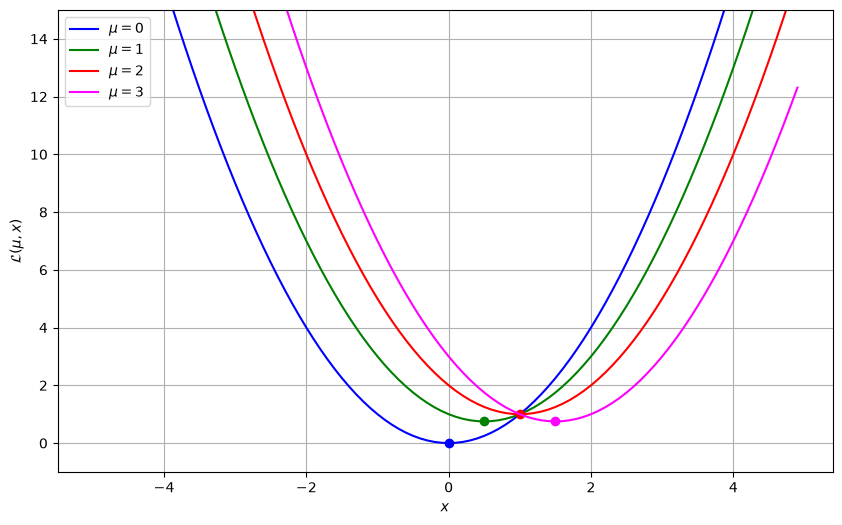
\includegraphics[width=0.9\linewidth]{imgs/1.png}
            \caption{Lagrangian with different $\mu$'s, with minimum of each indicated.}
            \label{diffmus}
        \end{figure}

        It can be seen that as $\mu$ increases, the minimizer keeps moving to the right.

        To see this analytically, note that for some fixed $\mu$, $\mathcal{L}\left( x, \mu \right)$ is a quadratic of $x$ and with a minimum where \[
            \der{\mathcal{L}\left( x, \mu \right)}{x} = 2x - \mu = 0,
        \] i.e., at $x = \frac{\mu}{2}$, showing that the minimizer does indeed move to the right with increasing $\mu$.

        \item \label{q1b} We formulate the dual function as \[
            d \left( \mu \right)
            =
            \min_{x} \mathcal{L} \left( \mu, x \right)
            =
            \mathcal{L} \left( \mu, \dfrac{\mu}{2} \right)
            =
            \mu - \dfrac{\mu^2}{4}.
        \] A plot of the function with its maximum also indicated is given in Figure \ref{dual}.

        \begin{figure}[H]
            \centering
            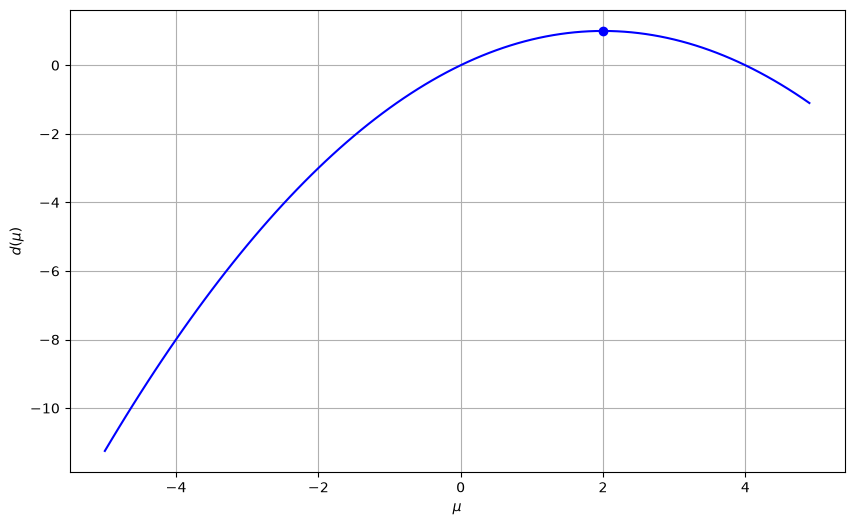
\includegraphics[width=0.9\linewidth]{imgs/2.png}
            \caption{The dual problem and its maximum.}
            \label{dual}
        \end{figure}

        The maximum occurs at $\left(2, 1\right)$, so \[
            \mu^\star = \underset{\mu \geq 0}{\arg \max}\, d\left( \mu \right)
            =
            2,
        \] and \[
            d^\star = \max_{\mu \geq 0}\, d\left( \mu \right) = 1.
        \]
        
        \item \label{q1c} For given $x$, $\mathcal{L}$ is a linear function of $\mu$. When $1 - x > 0$, $\mathcal{L}\left(\mu, x\right)$ is maximized by letting $\mu \to \infty$, which causes $\mathcal{L}\left(\mu, x\right) \to \infty$ as well, but when $1 - x < 0$, it is maximized by letting $\mu \to -\infty$.
        
        However, we are constrained by the inequality $\mu \geq 0$, so the maximum actually achievable in the latter case is $x^2$, with $\mu = 0$.

        Hence, \[
            g \left( x \right)
            =
            \max_{\mu \geq 0} \mathcal{L}\left(\mu, x\right)
            =
            \begin{cases}
                \infty, & \text{when } x < 1 \\
                x^2,    & \text{otherwise}.
            \end{cases}
        \] A visual representation of $g$ is given in Figure \ref{g}.

        \begin{figure}[H]
            \centering
            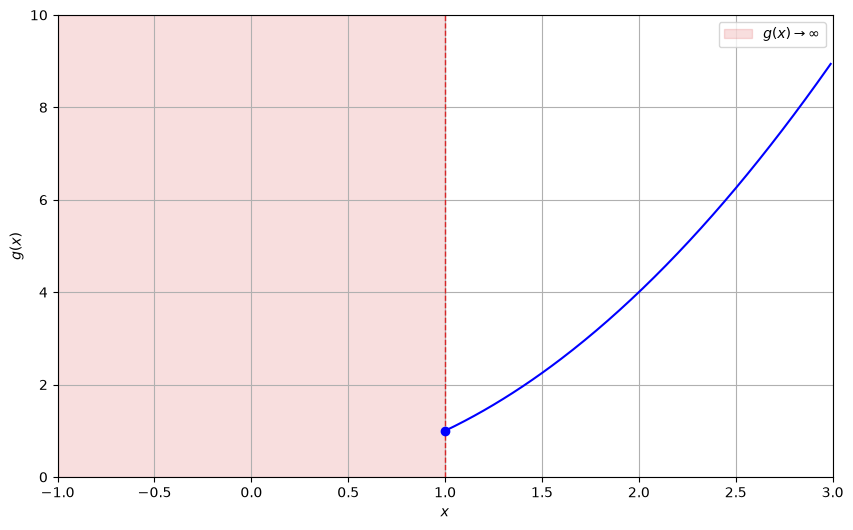
\includegraphics[width=0.9\linewidth]{imgs/3.png}
            \caption{$g(x)$.}
            \label{g}
        \end{figure}

        Now the minimum of this function clearly does not occur anywhere in the region with $x < 1$, and may only occur in the region with $x \geq 1$. But for $x \geq 1$, the value of the function is precisely $x^2$. 
        
        Therefore, minimizing $g(x)$ is equivalent to looking for the minimum of $x^2$, with $x \geq 1$. In other words, the problems \[
            \min_x g\left( x \right)
            \quad
            \text{ and }
            \quad
            \min_{x} x^2 \text{ subject to } x \geq 1
        \] are equivalent.

    \end{enumerate}

    \subsection*{Question 02}
    \begin{enumerate}[label=(\alph*), ref=2.\alph*]
        \item \label{q2a} We will show that $\mu^\star = 2$ and $x^\star = 1$ satisfy \[
            \mathcal{L} \left( \mu, x^\star \right)
            \leq
            \mathcal{L} \left( \mu^\star, x^\star \right)
            \leq
            \mathcal{L} \left( \mu^\star, x \right),
        \] for all $x$ and $\mu \geq 0$.
        
        \begin{enumerate}[label=(\roman*), ref=\theenumi.\roman*]
            \item \label{q2a_i}
            \begin{align*}
                \mathcal{L}\left( \mu^\star, x^\star \right)
                &=  \mathcal{L}\left( 2, 1 \right) \\
                &=  1^2 + 2 \cdot \left( 1 - 1 \right) = 1.
            \end{align*}
            
            \item \label{q2a_ii}
            \begin{align*}
                \mathcal{L}\left( \mu, x^\star \right)
                &=  \mathcal{L}\left( \mu, 1 \right) \\
                &=  1^2 + \mu \cdot \left( 1 - 1 \right) = 1,
            \end{align*}
            which is a constant function and does not depend on $\mu$.

            $1 \leq 1$, so this establishes the left inequality.
            
            \item \label{q2a_iii}
            \begin{align*}
                \mathcal{L}\left( \mu^\star, x \right)
                &=  \mathcal{L}\left( 2, x \right) \\
                &=  x^2 + 2 \cdot \left( 1 - x \right) \\
                &=  \left( x^2 - 2x + 1 \right) + 1 \\
                &=  \left( x - 1 \right)^2 + 1.
            \end{align*}

            For all $x$, $\left( x - 1 \right)^2 \geq 0$. Adding $1$ to both sides and rearranging gives $1 \leq \left( x - 1 \right)^2 + 1$, hence establishing the right inequality above.

            \item \label{q2a_iv} Figure \ref{ineq1} shows plots of $\mathcal{L}\left( \mu, x^\star \right)$ against $\mu$, and $\mathcal{L}\left( \mu^\star, x \right)$ against $x$, with the optimum points also indicated.
            
            \begin{figure}[H]
                \centering
                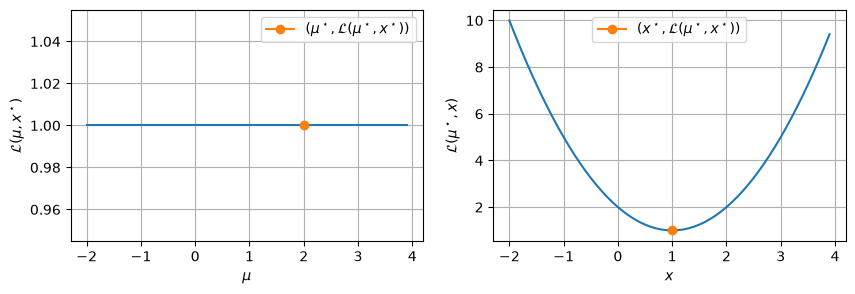
\includegraphics[width=0.9\linewidth]{imgs/4.png}
                \caption{Plots of $\mathcal{L}\left( \mu, x^\star \right)$ and $\mathcal{L}\left( \mu^\star, x \right)$, with the optimum points indicated.}
                \label{ineq1}
            \end{figure}

        \end{enumerate}
        
        \item \label{q2b} We assume that $f$ and $h$ are convex to establish the results.
        
        For each equality/inequality, we provide a one-line reason at the start, and go into further detail below.

        \begin{enumerate}[label=(\arabic*), ref=\theenumi.\arabic*]
            \item \label{q2b1} \textit{Complementary slackness.}
            
            There are two cases; (1) the inequality constraint is active at $x^\star$, so that $h\left( x^\star \right) = 0$, and (2) the inequality constraint is inactive, so $h\left( x^\star \right) < 0$.
            
            We consider each case in turn.
            
            In case (1), \[
                \mathcal{L}\left( \mu, x^\star \right)
                =
                f\left( x^\star \right) + \mu h\left( x^\star \right)
                =
                f\left( x^\star \right) + \mu \cdot 0 = f\left( x^\star \right)
            \] for any $\mu$, including $\mu = \mu^\star$, so \[
                f\left( x^\star \right)
                =
                \mathcal{L}\left( \mu^\star, x^\star \right).
            \]

            In case (2), note that the dual function may be written \[
                d\left( \mu \right)
                =
                \min_x \mathcal{L} \left( \mu, x \right)
                =
                f\left( x_\mu \right) + \mu h\left( x_\mu \right),
            \] where $x_\mu$ is the corresponding minimizer for the given $\mu$. Clearly then, for arbitrary $x$ that is not necessarily $x_\mu$, \[
                d\left( \mu \right) \leq f\left( x \right) + \mu h\left( x \right),
            \] including particularly when $x = x^\star$, giving \[
                d\left( \mu \right)
                \leq
                f\left( x^\star \right) + \mu h\left( x^\star \right)
                =
                \mathcal{L}\left( \mu, x^\star \right).
            \] Viewing everything now as functions of $\mu$, we have just shown that $d\left( \mu \right)$ is bounded above by $\mathcal{L}\left( \mu, x^\star \right)$, which is linear in $\mu$ with negative slope, because $h\left( x^\star \right) < 0$.

            Consider when $\mu = 0$. Then, \[
                d\left( 0 \right)
                =
                \min_x \mathcal{L} \left( 0, x \right)
                =
                \min_x f\left( x \right),
            \] is the global minimizer of $f$.
            
            Now the optimal solution to the primal problem is $x^\star$, and the inequality constraint is inactive there.

            If $f$ is convex and has only one global minimum (as we have assumed to be the case here), the fact that the inequality constraint is inactive there means that it plays no role in the problem, and might as well be excluded. In other words, the problems \[
                \min_x f\left( x \right)
                \quad
                \text{ and }
                \quad
                \min_{x} f\left( x \right) \text{ subject to } h\left( x \right) \leq 0
            \] are equivalent. Hence, if the $x$ which solves the latter problem is $x^\star$, then it is also the global minimizer of $f$, and it follows that \[
                d\left( 0 \right)
                =
                \min_x f\left( x \right)
                =
                f\left( x^\star \right)
                =
                \mathcal{L}\left( 0, x^\star \right).
            \]
            
            Now for any $\mu$ greater than $0$, $\mathcal{L}\left( \mu, x^\star \right) < \mathcal{L}\left( 0, x^\star \right)$, as $\mathcal{L}$ is decreasing linearly in $\mu$. At $\mu = 0$, $d\left( 0 \right)$ is exactly equal to $\mathcal{L}\left( 0, x^\star \right)$, and can never be any bigger for any $\mu > 0$, as it would then be bounded by a smaller number.
            
            The optimal $\mu$ therefore must be $0$; \[
                \mu^\star
                =
                \underset{\mu \geq 0}{\arg \max} \, d\left( \mu \right)
                =
                0.
            \] Hence, \[
                \mathcal{L}\left( \mu^\star, x^\star \right)
                =
                f\left( x^\star \right) + 0 \cdot h\left( x^\star \right)
                =
                f\left( x^\star \right).
            \]

            We have established the required equality in both cases.

            \item \textit{Right saddle-point inequality.}
            
            \label{q2b2} We consider the same two cases as above.
            
            In case (1), we start by defining the following set, which describes a region in space: \[
            R = \left\{
                \left( u, v \right)
                :
                \text{there exists } x \text{ s.t. } h\left( x \right) \leq u \text{ and } f\left( x \right) \leq v
            \right\}.
            \] Note that $R$ is a convex set when both $f$ and $h$ are convex.
            
            We seek the lowermost point of $R$ in the left half plane, where $h\left( x \right) \leq u \leq 0$. The $x$ which leads to that point is the solution to the primal problem.
            
            Now when the primal solution is such that $h\left( x^\star \right) = 0$, $R$ must contain a point with $u = 0$. When $u = 0$, i.e., when $h(x) \leq 0$, the least $f$ can be is $f\left( x^\star \right)$, so $v$ can be at least $f\left( x^\star \right)$.
            
            Hence, $R$ must contain the point $\left( 0, f\left( x^\star \right) \right)$, and it must also be the lowermost point of $R$ in the left half plane, for if not there should exist a more optimal solution. % with the constraint inactive ?? apparently not necessarily?? 

            We would like to draw a line through this point, given by \[
                pu + qv = r
            \] for $p, q \geq 0$ such that $R$ lies entirely above it and to its right (the supporting hyperplane).

            As the line must pass $\left( 0, f\left( x^\star \right) \right)$, we find that $r = q f\left( x^\star \right)$, so that the line is \[
                pu + qv = q f\left( x^\star \right).
            \]

            Now, assuming that the left half of the plane is not empty, i.e., there is at least one $\hat{x}$ such that $h\left( \hat{x} \right)$ is strictly less than, and not equal to $0$, we eliminate the possibility that $q = 0$; because if $q = 0$, then the line becomes vertical, restricting $R$ entirely to the right half plane.

            Knowing that $q \ne 0$, we can now divide through by $q$, and let $\hat{\mu} = \dfrac{p}{q} \geq 0$ to get the equation of the line as \[
                \left( \dfrac{p}{q} \right) u + v
                =
                \hat{\mu} u + v
                =
                f\left( x^\star \right).
            \]

            This line always lies below $R$, so any $\left( u, v \right) \in R$ satisfies \[
                \hat{\mu} u + v
                \geq
                f\left( x^\star \right).
            \]

            Now $u$ is a number such that $h\left( x \right) \leq u$ for some $x$, and $v$ is a number such that $f\left( x \right) \leq v$ for some $x$. $h\left( x \right) \leq h\left( x \right) = u$ is trivially true, as is $f\left( x \right) \leq f\left( x \right) = v$. Hence, for any $x$, we have \[
                \hat{\mu} h\left( x \right) + f\left( x \right)
                =
                f\left( x \right) + \hat{\mu} h\left( x \right)
                =
                \mathcal{L}\left( \hat{\mu}, x \right)
                \geq
                f\left( x^\star \right).
            \] Note that the result holds for any arbitrary $x$. In other words then, we have shown that $f\left( x^\star \right)$ is a lower bound for $\mathcal{L}\left( \hat{\mu}, x \right)$ over all $x$.
            
            But the largest lower bound for $\mathcal{L}\left( \hat{\mu}, x \right)$ is given by the dual function $d\left( \hat{\mu} \right)$. Hence, we have \[
                d\left( \hat{\mu} \right) \geq f\left( x^\star \right).
            \]

            By definition of the dual function, it is always true that for any arbitrary $x$, including precisely when $x = x^\star$, we have \[
                d\left( \hat{\mu} \right)
                \leq
                f\left( x^\star \right) + \hat{\mu} h\left( x^\star \right)
                =
                f\left( x^\star \right).
            \]
            
            These two inequalities together give $d\left( \hat{\mu} \right) = f\left( x^\star \right)$.

            Note that the result $d\left( \mu \right) \leq f\left( x^\star \right)$ holds for all $\mu$. The largest value that $d$ may achieve over any $\mu$ is therefore $f\left( x^\star \right)$, and if there exists any $\mu$ where it equals $f\left( x^\star \right)$ exactly, it is a maximizer of $d$ over $\mu$.

            We have just shown that $d\left( \hat{\mu} \right) = f\left( x^\star \right)$, so $\hat{\mu}$ is a maximizer of $d$. % this is sorta saying uniqueness of mustar, but that is not true. i mean its just any maximizer. maybe there are several maximizers all giving same answer. *the* mustar may not be muhat, but just maximizer works.

            We showed earlier that \[
                \mathcal{L}\left( \hat{\mu}, x \right)
                \geq
                f\left( x^\star \right),
            \] and because $\mu^\star$ is also a maximizer of $d$, the same result holds if we replace $\hat{\mu}$ with $\mu^\star$, i.e., \[
                \mathcal{L}\left( \mu^\star, x \right)
                \geq
                f\left( x^\star \right)
                =
                f\left( x^\star \right) + \mu^\star \cdot 0
                =
                f\left( x^\star \right) + \mu^\star \cdot h\left( x^\star \right)
                =
                \mathcal{L}\left( \mu^\star, x^\star \right).
            \]

            In case (2), the same arguments shown in the previous problem apply, and $\mu^\star = 0$. If $f$ is convex and has only a single minimum, $f\left( x^\star \right)$ is less than or equal $f\left( x \right)$ for any $x$, so \[
                \mathcal{L}\left( \mu^\star, x^\star \right)
                =
                f\left( x^\star \right) + 0 \cdot h\left(x^\star\right)
                =
                f\left( x^\star \right)
                \leq
                f\left( x \right)
                =
                \mathcal{L}\left( \mu^\star, x \right).
            \]

            Hence, we have shown that the inequality holds in both cases.
            
            \item \label{q2b3} This is simply the definition of $\mathcal{L}$. $\mathcal{L}\left( \mu^\star, x \right) = f\left( x \right) + \mu^\star h\left( x \right)$.
            
            \item \label{q2b4} For any feasible $x$, $h\left( x \right) \leq 0$. By definition, $\mu^\star \geq 0$. Hence, $\mu^\star h\left( x \right) \leq 0$ trivially. Adding $f\left( x \right)$ to both sides gives the desired result.
        \end{enumerate}

        The inequality $\mathcal{L}\left( \mu, x^\star \right) \leq \mathcal{L}\left( \mu^\star, x^\star \right)$ requires that $\mathcal{L}\left( \mu, x^\star \right)$ be less than or equal to a finite number as $\mu$ is varied over non-negative values.

        But $\mathcal{L}\left( \mu, x^\star \right) = f\left( x^\star \right) + \mu h\left( x^\star \right)$. If $h\left( x^\star \right) > 0$, then as $\mu \to \infty$, $\mathcal{L}\left( \mu, x^\star \right) \to \infty$ as well, contradicting the inequality. Hence, we must have $h\left( x^\star \right) \leq 0$.
        
        If $h\left( x^\star \right) < 0$, then as $\mu \to \infty$, $\mathcal{L}\left( \mu, x^\star \right) \to -\infty$. It will remain bounded above by a finite number, but by itself will decrease without bound.

        Hence, if we also require $\mathcal{L}\left( \mu, x^\star \right)$ to remain finite as $\mu \to \infty$, the only possibility is that $h\left( x^\star \right) = 0$.
        
        \item \label{q2c} We have shown complementary slackness in case (1) above.
        
        If $h\left( x^\star \right) = 0$, then for any $\mu$, including $\mu^\star$, $\mu^\star h\left( x^\star \right) = 0$. If instead $h\left( x^\star \right) < 0$, then $\mu^\star = 0$, and we still have $\mu^\star h\left( x^\star \right) = 0$.

        If the constraint changes to $x \geq -1$, the solution is $x^\star = 0$; exactly the same as that for the unconstrained problem. $h\left( x^\star \right) = -1 - x^\star = -1 \leq 0$, so it is indeed feasible, but because $h\left( x^\star \right) \ne 0$, the constraint is inactive there.

        As the constraint is inactive, we expect $\mu^\star = 0$ by complementary slackness.
    \end{enumerate}

    \subsection*{Question 03}
    \begin{enumerate}[label=(\alph*), ref=3.\alph*]
        \item \label{q3a}
        \begin{enumerate}[label=(\arabic*), ref=\theenumi.\arabic*]
            \item \label{q3a1} By definition, \[
                d\left( \mu \right)
                =
                \min_x \mathcal{L}\left( \mu, x \right).
            \] It is the least value that $\mathcal{L}\left( \mu, x \right)$ takes over all $x$, for that given $\mu$. Hence, for arbitrary $x$, we have \[
                d\left( \mu \right)
                \leq
                \mathcal{L}\left( \mu, x \right).
            \]

            \item \label{q3a2} If $x$ is feasible, then $h\left( x \right) \leq 0$. By definition, $\mu \geq 0$. Hence, $\mu h\left( x \right) \leq 0$. Adding $f\left( x \right)$ to both sides gives \[
                f\left( x \right) + \mu h\left( x \right) \leq f\left( x \right).
            \]
        \end{enumerate}

        Chaining the two inequalities gives \[
            d\left( \mu \right) \leq f\left( x \right),
        \] and when $x = x^\star$, we get \[
            d\left( \mu \right) \leq f\left( x^\star \right) = p^\star.
        \]

        In Question \ref{q1a}, we specifically found that $d\left( 0 \right) = 0$, $d\left( 1 \right) = 0.75$, $d\left( 2 \right) = 1$ and $d\left( 3 \right) = 0.75$. $p^\star = 1$ here, and all the above values are clearly less than or equal to $1$.
        
        \item \label{q3b} Figure \ref{lofmu} shows plots of $\mathcal{L}\left( \mu, x \right)$ as a functions of $\mu$, for various $x = 0, 1, 2$. The envelope formed by the minimum points of the lines, and a plot of the actual $d\left( \mu \right)$ are also shown.
        
        The envelope of the three lines forms a concave shape. As more lines are added, the shape of $d\left( \mu \right)$ will be seen to emerge.
        
        \begin{figure}[H]
            \centering
            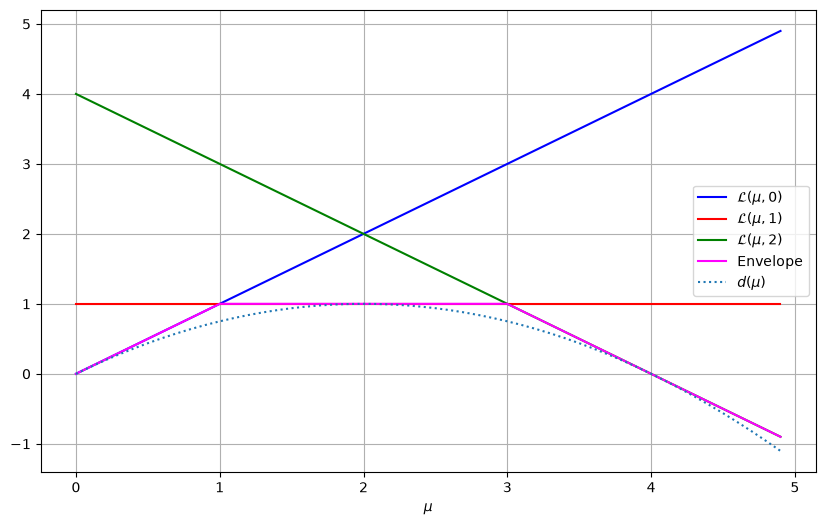
\includegraphics[width=0.9\linewidth]{imgs/5.png}
            \caption{$\mathcal{L}\left( \mu, x \right)$ as a function of $\mu$ for various $x$.}
            \label{lofmu}
        \end{figure}

        For any $f$, the value of $d\left( \mu \right)$ is the minimum point of a series of straight lines linear in $\mu$. Such a curve will always be concave.

        More technically, let $\mu_1$ and $\mu_2$ be any two arbitrary $\mu$'s. Let $\bar{\mu} = t \mu_1 + \left( 1 - t\right) \mu_2$, for $t \in \left[ 0, 1\right]$.

        Then, $d\left( \bar{\mu }\right) = f\left( x_{\bar{\mu }} \right) + \bar{\mu} h\left( x_{\bar{\mu}} \right) = \mathcal{L}\left( \bar{\mu}, x_{\bar{\mu}} \right)$.
        
        Consider now the straight line given by $\mathcal{L}\left( \mu, x_{\bar{\mu}} \right)$. We must have \[
            d\left( \bar{\mu} \right)
            =
            \mathcal{L}\left( \bar{\mu}, x_{\bar{\mu}} \right)
            =
            \mathcal{L}\left( t \mu_1 + \left( 1 - t\right) \mu_2, x_{\bar{\mu}} \right)
            =
            t \mathcal{L}\left( \mu_1, x_{\bar{\mu}} \right)
            +
            \left( 1 - t \right) \mathcal{L}\left( \mu_2, x_{\bar{\mu}} \right)
        \] by linearity. But by definition of $d\left( \mu \right)$, we also have \[
            d\left( \mu_1 \right) \leq \mathcal{L}\left( \mu_1, x_{\bar{\mu}} \right)
            \quad
            \text{and}
            \quad
            d\left( \mu_2 \right) \leq \mathcal{L}\left( \mu_2, x_{\bar{\mu}} \right),
        \] and because $t, 1 - t \geq 0$, \[
            d\left( \bar{\mu} \right)
            =
            d\left( t \mu_1 + \left( 1 - t\right) \mu_2 \right)
            =
            t \mathcal{L}\left( \mu_1, x_{\bar{\mu}} \right)
            +
            \left( 1 - t \right) \mathcal{L}\left( \mu_2, x_{\bar{\mu}} \right)
            \geq
            t d\left( \mu_1 \right)
            +
            \left( 1 - t \right) d\left( \mu_2 \right),
        \] which is precisely the definition of concavity.
    \end{enumerate}


\end{document}